\documentclass[a4paper]{article}

%% Language and font encodings
% \usepackage[english]{babel}
% \usepackage[T1]{fontenc}

%% Sets page size and margins
\usepackage[a4paper,top=3cm,bottom=2cm,left=3cm,right=3cm,marginparwidth=1.75cm]{geometry}
\usepackage{amsmath}
\usepackage{mathtools}
\usepackage{graphicx}
\graphicspath {{images/}}

\title{CS698 - Winter 2017 - Assignment 1}
\author{Vineet John (v2john@uwaterloo.ca)}
\date{}


\begin{document}
\maketitle

\renewcommand\thesubsection{\alph{subsection}}

\section{Classification}

The code for the K Nearest Neighbours implementation is contained in the zip file `k-nearest-neighbours-code.zip'. The command to run the code is present in the README.md file.
\\\\
The plot in Figure \ref{fig_classification_accuracy} is a measure of accuracy vs. k. The best k found was 20, which is represented by the highest point on the curve.

\begin{figure*}[h]
    \centering
    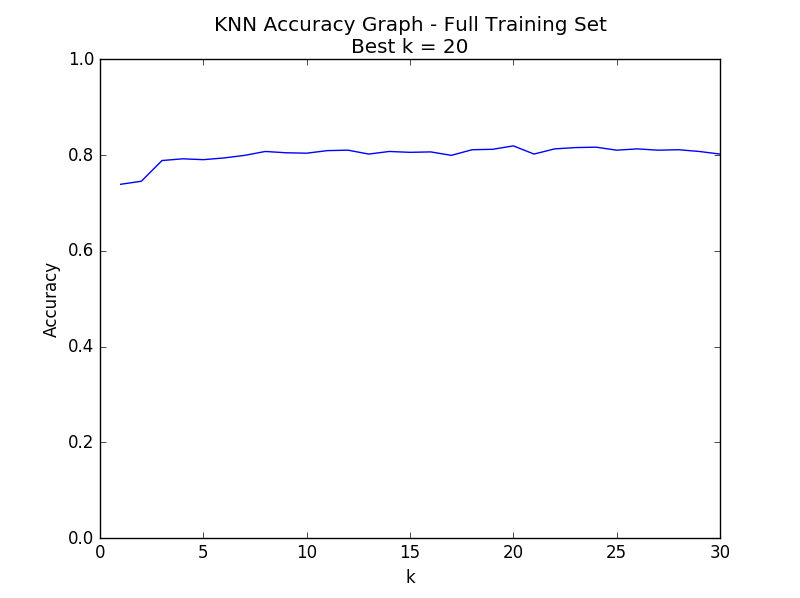
\includegraphics[width=\textwidth]{images/knn_accuracy_crossval.png}
    \caption{Classification Accuracy}
    \label{fig_classification_accuracy}
\end{figure*}

\newpage

\section{Regression}

The code for the Linear Regression implementation is contained in the zip file `linear-regression-code.zip'. The command to run the code is present in the README.md file.
\\\\
Since the penalty term is $\lambda w^Tw$, the final expression to evaluate for the linear regression will be $(2\lambda I + A)w = b$, where $A = \sum_{n=1}^N \bar{x}_n \bar{x}_n^T$ and $b = \sum_{n=1}^N t_n \bar{x}_n$
\\\\
The plot in Figure \ref{fig_regression_accuracy} is a measure of euclidean loss vs. the regularization parameter $\lambda$. The best $\lambda$ found was 0.6, which is represented by the lowest point on the curve.


\begin{figure*}[h]
    \centering
    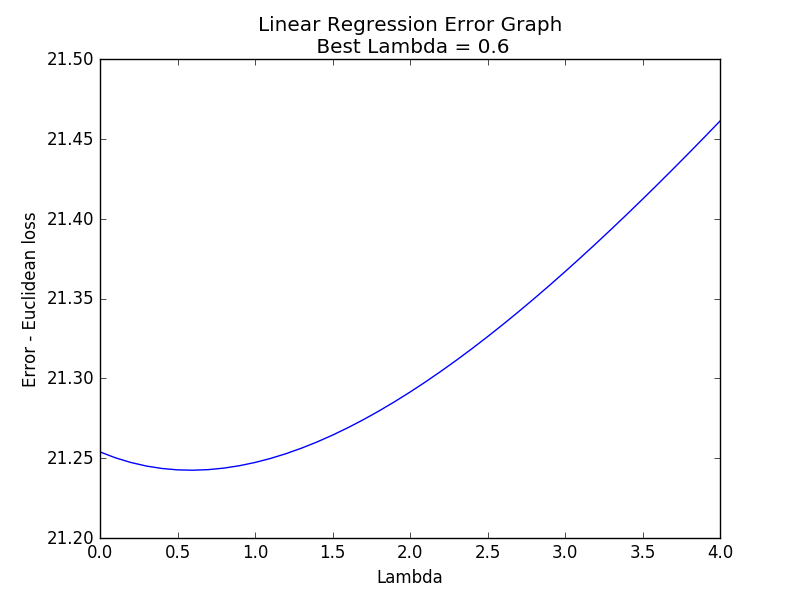
\includegraphics[width=\textwidth]{images/linear_regression_accuracy.png}
    \caption{Regression Accuracy}
    \label{fig_regression_accuracy}
\end{figure*}

\newpage

\section{Theory}

\subsection{Derive a closed-form expression for the estimates of w and b that minimize the objective}

\subsubsection{Problem Statement}

Theory. In class, we discussed several loss functions for linear regression. However all the loss functions that we discussed assume that the error contributed by each data point have the same importance. Consider a scenario where we would like to give more weight to some data points. Our goal is to fit the data points $(x_n , y_n )$ in proportion to their weights $r_n$ by minimizing the following objective:

$$L(w, b) = \sum_{n=1}^m r_n (y_n - wx_n + b)^2$$


\subsubsection{Calculation of the partial derivatives}

Since the loss function needs to be minimized with respect to 2 variables, the partial derivative of the loss function L with respect to each variable is calculated independently.

\begin{align*}
	\frac{\partial L}{\partial w} &= 0\\
	2 * \sum_{n=1}^m r_n (y_n - wx_n + b) x_n &= 0\\
	\sum_{n=1}^m r_n (y_n - wx_n + b) x_n &= 0\\
	\sum_{n=1}^m r_n (y_n x_n - wx_nx_n^T + bx_n) &= 0\\
	\sum_{n=1}^m r_n y_n x_n - r_n w x_n x_n^T + r_n b x_n &= 0\\
	\sum_{n=1}^m r_n y_n x_n - w \sum_{n=1}^m r_n x_n x_n^T + b \sum_{n=1}^m r_n x_n &= 0\\
	w \sum_{n=1}^m r_n x_n x_n^T &=  \sum_{n=1}^m r_n y_n x_n + b \sum_{n=1}^m r_n x_n
\end{align*}

\begin{align}
\label{pd_w}
	\Aboxed{w  = \frac{b \sum_{n=1}^m r_n x_n + \sum_{n=1}^m r_n y_n x_n} {\sum_{n=1}^m r_n x_n x_n^T}}
\end{align}

\vspace{5mm}

Also, 

\begin{align*}
	\frac{\partial L}{\partial b} &= 0\\
	2 * \sum_{n=1}^m r_n (y_n - w x_n + b) &= 0\\
	\sum_{n=1}^m r_n (y_n - w x_n + b) &= 0\\
	\sum_{n=1}^m r_n (y_n - w x_n + b) &= 0\\
	\sum_{n=1}^m r_n y_n - r_n w x_n + r_n b &= 0\\
	\sum_{n=1}^m r_n y_n - w \sum_{n=1}^m r_n x_n + b \sum_{n=1}^m r_n &= 0\\
	b \sum_{n=1}^m r_n &= w \sum_{n=1}^m r_n x_n - \sum_{n=1}^m r_n y_n
\end{align*}

\begin{align}
\label{pd_b}
	\Aboxed{b = \frac{w \sum_{n=1}^m r_n x_n - \sum_{n=1}^m  r_n y_n}{\sum_{n=1}^m  r_n}}
\end{align}


\subsubsection{Solution of the system of linear equations}

The value of b, as obtained in Equation \ref{pd_b} is substituted in Equation \ref{pd_w}.

\begin{align*}
	w &= \frac{\frac{w \sum_{n=1}^m r_n x_n - \sum_{n=1}^m r_n y_n}{\sum_{n=1}^m r_n} \sum_{n=1}^m r_n x_n + \sum_{n=1}^m r_n y_n x_n} {\sum_{n=1}^m r_n x_n x_n^T}\\
	w &= \frac{(w \sum_{n=1}^m r_n x_n - \sum_{n=1}^m r_n y_n) \sum_{n=1}^m r_n x_n + \sum_{n=1}^m r_n y_n x_n \sum_{n=1}^m r_n} {\sum_{n=1}^m r_n x_n x_n^T \sum_{n=1}^m r_n}\\
	w &= \frac{w ({\sum_{n=1}^m r_n x_n})^2 - \sum_{n=1}^m r_n y_n \sum_{n=1}^m r_n x_n + \sum_{n=1}^m r_n y_n x_n \sum_{n=1}^m r_n} {\sum_{n=1}^m r_n x_n x_n^T \sum_{n=1}^m r_n}\\
	w \sum_{n=1}^m r_n x_n x_n^T \sum_{n=1}^m  r_n &= w ({\sum_{n=1}^m r_n x_n})^2 - \sum_{n=1}^m  r_n y_n \sum_{n=1}^m  r_n x_n + \sum_{n=1}^m  r_n y_n x_n \sum_{n=1}^m  r_n\\
	w \sum_{n=1}^m r_n x_n x_n^T \sum_{n=1}^m  r_n - w ({\sum_{n=1}^m r_n x_n})^2 &= - \sum_{n=1}^m  r_n y_n \sum_{n=1}^m  r_n x_n + \sum_{n=1}^m  r_n y_n x_n \sum_{n=1}^m  r_n\\
	w (\sum_{n=1}^m r_n x_n x_n^T \sum_{n=1}^m  r_n - ({\sum_{n=1}^m r_n x_n})^2) &= - \sum_{n=1}^m  r_n y_n \sum_{n=1}^m  r_n x_n + \sum_{n=1}^m  r_n y_n x_n \sum_{n=1}^m  r_n\\
\end{align*}

\begin{align}
\label{cf_w}
	\Aboxed{w  = \frac{\sum_{n=1}^m  r_n y_n x_n \sum_{n=1}^m  r_n - \sum_{n=1}^m  r_n y_n \sum_{n=1}^m  r_n x_n}{\sum_{n=1}^m r_n x_n x_n^T \sum_{n=1}^m  r_n - ({\sum_{n=1}^m r_n x_n})^2}}
\end{align}

\vspace{10mm}

Now that the value of $w$ has been expressed in terms of $r_n$, $x_n$ and $y_n$, we can substitute this value of w in Equation \ref{pd_b} to obtain a closed form expression for $b$.

\begin{align*}
	b &= \frac{w \sum_{n=1}^m r_n x_n - \sum_{n=1}^m  r_n y_n}{\sum_{n=1}^m  r_n} \\
	b \sum_{n=1}^m  r_n &= w \sum_{n=1}^m r_n x_n - \sum_{n=1}^m  r_n y_n\\
	b \sum_{n=1}^m  r_n &= \frac{\sum_{n=1}^m  r_n y_n x_n \sum_{n=1}^m  r_n - \sum_{n=1}^m  r_n y_n \sum_{n=1}^m  r_n x_n}{\sum_{n=1}^m r_n x_n x_n^T \sum_{n=1}^m  r_n - ({\sum_{n=1}^m r_n x_n})^2} \sum_{n=1}^m r_n x_n - \sum_{n=1}^m  r_n y_n\\
	b \sum_{n=1}^m  r_n &= \frac{\sum_{n=1}^m  r_n y_n x_n \sum_{n=1}^m  r_n - \sum_{n=1}^m  r_n y_n \sum_{n=1}^m  r_n x_n}{\sum_{n=1}^m r_n x_n x_n^T \sum_{n=1}^m  r_n - ({\sum_{n=1}^m r_n x_n})^2} \sum_{n=1}^m r_n x_n - \sum_{n=1}^m  r_n y_n\\
	b \sum_{n=1}^m  r_n &= \frac{\sum_{n=1}^m  r_n y_n x_n \sum_{n=1}^m  r_n \sum_{n=1}^m r_n x_n - \sum_{n=1}^m  r_n y_n (\sum_{n=1}^m  r_n x_n)^2}{\sum_{n=1}^m r_n x_n x_n^T \sum_{n=1}^m  r_n - ({\sum_{n=1}^m r_n x_n})^2} - \sum_{n=1}^m  r_n y_n
\end{align*}

\begin{align}
\label{cf_b}
	\Aboxed{b &= \frac{\sum_{n=1}^m r_n y_n x_n \sum_{n=1}^m r_n \sum_{n=1}^mr_n x_n - \sum_{n=1}^m r_n y_n (\sum_{n=1}^m r_n x_n)^2}{\sum_{n=1}^mr_n x_n x_n^T (\sum_{n=1}^m r_n)^2 - \sum_{n=1}^m r_n ({\sum_{n=1}^mr_n x_n})^2} - \frac{\sum_{n=1}^m r_n y_n}{\sum_{n=1}^m r_n}}
\end{align}

\vspace{5mm}

\subsubsection{Conclusion}
Equations \ref{cf_w} and \ref{cf_b} are the closed form solutions for minimizing the loss function L, in terms of the input variable x, the target variable w, and the local weight r.

\newpage


\subsection{Equivalence to the negative log-likelihood for linear regression}

\subsubsection{Problem Statement}

Show that this objective is equivalent to the negative log-likelihood for linear regression where each data point may have a different Gaussian measurement noise. What is the variance of each measurement noise in this model?
$$L(w, b) = \sum_{n=1}^{\\m} r_n (y_n - wx_n + b)^2$$

\subsubsection{Solution}

Assume that linear regression problem is modeled such that $w^T\bar{x_n} - b$ is the prediction term rather than just $w^T\bar{x_n}$ as in the above equation.\\\\
Given that $y = f(x) + \epsilon$, where $\epsilon$ is the measurement error and $f(x)$ is the underlying function to be predicted, $f(x) = w^T\bar{x_n} - b$.\\
The measurement noise $\epsilon$ is assumed to be a Gaussian distribution such that $\epsilon = N(0, \sigma^2)$\\\\
Now, the probability of the target variable y, given the input parameters X, w and b can be denoted as: \\
\begin{align*}
	Pr(y|\bar{X},w,b,\sigma) &= N(y|w^T\bar{x_n} - b,\sigma)\\
	&= \prod_{n=1}^{N} \frac{1}{\sqrt{2\pi}\sigma} e ^{-\frac{(y - w^T\bar{x_n} + b)^2}{2\sigma^2}}
\end{align*}
\\
To obtain the optimal value of w and b, the maximum likelihood estimate is evaluated:
\begin{align*}
	w^*, b^* &= argmax_{w,b} Pr(y|\bar{X},w,b,\sigma_)\\
	&= \prod_{n=1}^{N} \frac{1}{\sqrt{2\pi}\sigma_n} e ^{-\frac{(y - w^T\bar{x_n} + b)^2}{2\sigma_n^2}}
\end{align*}
\\
Here, $\sigma_n$ denotes that each of the data-points has a different Gaussian measurement associated with it. 
\\
\\
Evaluating, the log of the maximum likelihood equation above,
\\
$$w^*, b^* = argmax_{w,b} \sum_{n=1}^{N} \frac{1}{\sqrt{2\pi}\sigma_n} * (-\frac{(y - w^T\bar{x_n} + b)^2}{2\sigma_n^2})$$
\\
Now, discarding the constant terms $\frac{1}{\sqrt{2\pi}}$ and $\frac{1}{2}$,
\\
\begin{align*}
	w^*, b^* &= argmax_{w,b} \sum_{n=1}^{N} \frac{1}{\sigma_n} * (-\frac{(y - w^T\bar{x_n} + b)^2}{2\sigma_n^2})\\
	&= argmax_{w,b} \sum_{n=1}^{N} \frac{1}{\sigma_n} * (-\frac{(y - w^T\bar{x_n} + b)^2}{\sigma_n^2})\\
	&= argmax_{w,b} \sum_{n=1}^{N} -\frac{(y - w^T\bar{x_n} + b)^2}{\sigma_n^3}\\
\end{align*}
Here, the standard deviation term $\sigma_n^3$ could be said to represent $r_n$, which models a distinct weight for each of the data-points.
\\
\\
Consequently, the final expression could be written as:\\
\begin{align}
\label{final-eq}
	\Aboxed{w^*, b^* &= argmin_{w,b} \sum_{n=1}^{N} r_n (y - w^T\bar{x_n} + b)^2}
\end{align}
which is the originial linear regression loss function, obtained from the negative log-likelihood of linear regression where each point has a different Gaussian measurement, with $\mu = 0$ and $variance = \sigma_i^2$ for a datapoint i.
\\
\\
The variance for this model can be evaluated by equating the assumption made in Equation \ref{final-eq}.
\begin{align*}
	\frac{1}{\sigma_n^3} &= r_n\\
	\sigma_n^3 &= r_n^{-1}
\end{align*}
\\
Equation \ref{eq-variance} gives the variance of each point in the model of linear regression where each point has a different Gaussian measurement.
\begin{align}
\label{eq-variance}
	\Aboxed{\sigma_n^2 &= r_n^{-2/3}}
\end{align}


\subsubsection{Conclusion}
The negative log-likelihood for linear regression, with each data point having a different Gaussian noise is proven to be the same as the objective with a different weight for each data point in the loss function, as shown in Equation \ref{final-eq}.\\
\\
Also, the variance of each point in the model is expressed in terms of the weight assigned in the weighted linear regression loss function, as shown in Equation \ref{eq-variance}.
\end{document}
